\documentclass[12pt]{article}
\usepackage{amsmath, amssymb, amsthm}
\usepackage{enumitem}
\usepackage{hyperref}
\usepackage{bm}
\usepackage[utf8]{inputenc}     % if you need it
\usepackage[T1]{fontenc}        % if you need it
\usepackage{subcaption}         % defines the subfigure environment
\usepackage{grffile}
\usepackage{placeins}    
\usepackage[a4paper,margin=1in]{geometry}
\usepackage{graphicx}
\usepackage{subcaption}  % for subfigure
\usepackage{float}       % for [H]
\usepackage{placeins}    % for \FloatBarrier

\hypersetup{
    colorlinks=true,
    linkcolor=blue,
    urlcolor=blue,
    citecolor=red
}
\begin{document}

\tableofcontents

\newpage
\section{Part A }
\subsection{Introduction and theoretical background}
\subsubsection{experiment goals}

For part A, we aim to verify the theory behind how electric and magnetic fields affect a moving electron.

\subsubsection{theory}
In this experiment, we study the effects of the electric and magnetic fields on a ray of electrons, more precisely on the direction of the beam.\\

A cathode ray tube is used to generate the electron beam. It works by heating a cathode to the temperature at which it starts to emit electrons. The electrons emitted are filtered by energy level and accelerated by two meshes, and then the beam is focused using two anodes.

\begin{figure}[h]
    \centering
    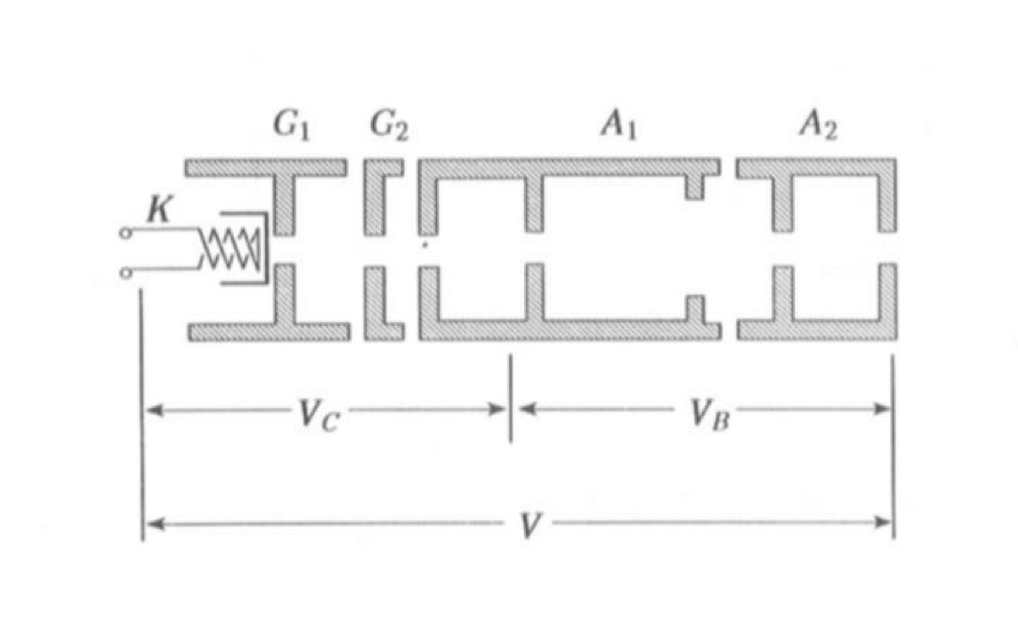
\includegraphics[width=0.5\linewidth]{ray gun diagram.png}
    \caption{ray tube diagram}
    \label{fig:CRT}
\end{figure} 
Where:
\begin{itemize}
    \item $K$ is the heated cathode.
    \item $G_1$ is the first mesh.
    \item $G_2$ is the second mesh.
    \item $A_1$ is the first anode. 
    \item $A_2$ is the second anode.
\end{itemize}
\par
From the diagram, we see that the first mesh acts as a physical barrier that only allows electrons emitted in a certain direction to go through; in addition, it also acts as a potential barrier also only allowing electrons with enough energy to pass, thus filtering the emitted electrons by direction of movement and energy. \\

The second mesh receives the electrons that were able to pass through the first mesh and accelerates them using a high voltage gate, thus, we get a group of electrons moving approximately in the right direction at high speeds. All we need to do now is concentrate them into a focused beam. \\

That is what the anodes are for, both anodes are charged tubes, the first anode slows down the electrons, and the second one speeds them up. The repetitive acceleration and deceleration of the electron beam focus it according to the electrostatic lens notion depicted in \ref{fig:lens}


To measure the effect of an electric field on the concentrated electron beam, a uniform electric field perpendicular to the beam is needed, which is done using a simple two-plate capacitor. The equation describing the electric field inside a two-plate capacitor is as follows: 

$$\vec{E} = - \frac{V_d}{d}$$
Where $d$ is the distance between the capacitors' plates

From electrodynamics, we know that under a constant electric field $\vec{E}$, an electron has an electric force working on it, equivalent in size to the electric field times the charge of the electron and opposite in direction to the electric field, and using newtons second law, we get:

\begin{equation}
    \vec{F} = -q_e E = \frac{eV_d}{d} 
    \Rightarrow \vec a =\frac{eV_d}{d m_e}
\end{equation}

Assuming that the electron is moving in the $\hat x$ direction and the acceleration is only in the $\hat y $ direction, it is possible to describe the deviation angle of the beam by the ratio of the initial velocity $\vec v_x$ and the acquired velocity $\vec v_y$.
\begin{equation} \label{2}
    \tan{\theta}=\frac{v_y}{v_x}
\end{equation}
where $\theta$ is the scattering angle of the electron beam. See \ref{fig: electron velocity in a cappacitor}
\\

And if the time the electrons spend under that acceleration is known and marked by $t$, we can find the velocity $\vec {v} _ y$ using simple kinematics. 

$$\vec v_y = \vec a_y \cdot t$$
Note that $t$ can be calculated from $l = v_x t$, considering the electron is spending little time in the capacitor, where $l$ is the length of the capacitor.\\

thus we can substitute $\vec{v}_y$ and $\vec{a}_y$ in \eqref{2} and get: 
\begin{equation} 
    \tan{\theta} = \frac{v_y}{v_x} = \frac{a_y l}{v_x^2} = \frac{eV_d l }{m v_x^2 d}
\end{equation}\\
The term apparent in the denominator, $mv_x^2$, is twice the kinetic energy of the electrons. From energy conservation we can say that the kinetic energy of the electron is equal to the potential energy that accelerated it at the beginning $eV$, not to be confused with $V_d$, which is the potential difference in the capacitor.
Thus we get: 
$$2eV = mv_x^2$$
\begin{equation} 
   \Rightarrow \tan{\theta} = \frac{V_d l }{2Vd}
\end{equation}
\textbf{The scattering angle of the electrons is determined only by the voltages applied in the CRT!}

\begin{figure}[h]
    \centering
    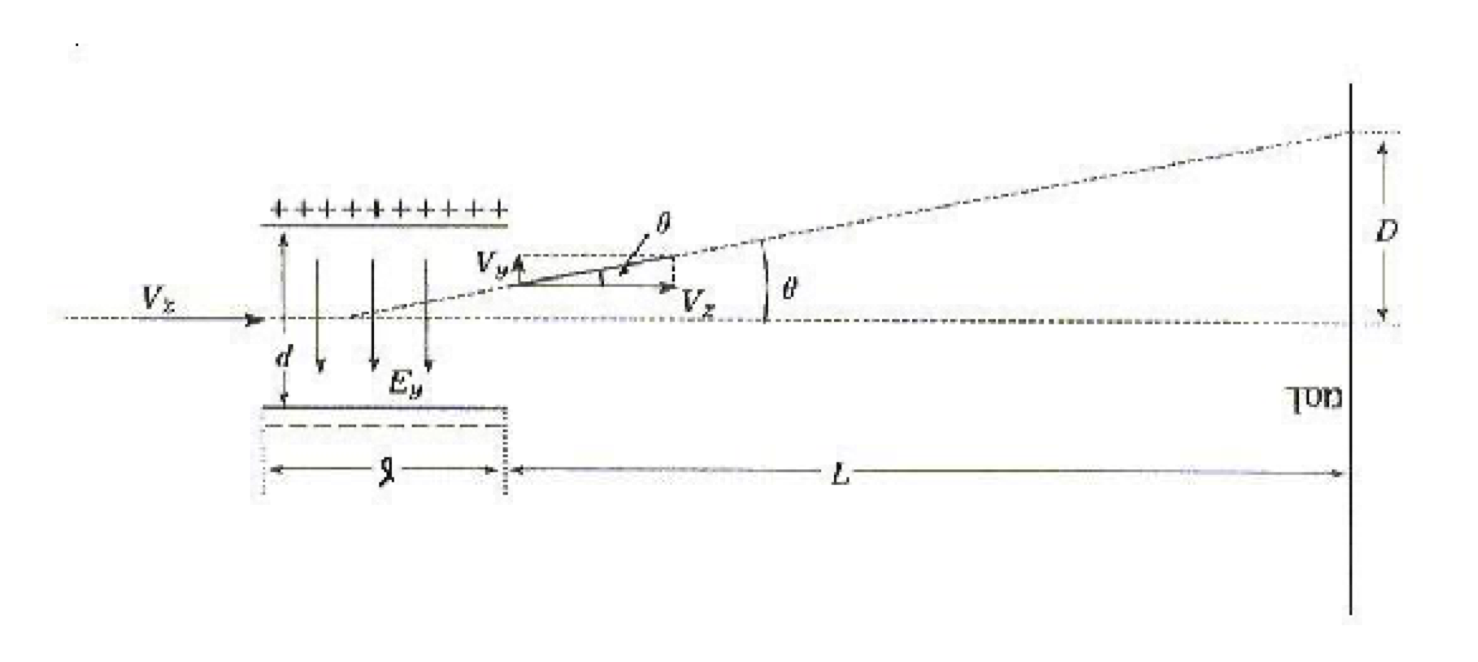
\includegraphics[width=0.5\linewidth]{electron velocity in a cappacitor.png}
    \caption{electron velocity in a cappacitor}
    \label{fig: electron velocity in a cappacitor}
\end{figure} 

Now, from simple geometry, we can see that: 
\begin{equation} \label{final theta}
    \tan{\theta} = \frac{D}{L + \frac l 2} = \frac{V_d l }{2Vd}
\end{equation}
Note that we consider that the scattering point is in the middle of the capacitor, which arises from the assumption that the force acted on the electrons is uniform throughout the capacitor and is always pointing in the $\hat y $ direction. \\

\textbf{For the second part of the experiment}, we want tot test the effect of a constqnt magnetic field on the electron beam.\\

In this expirement, a magnetic field is created using two spools of copper wire each with $n$ turns, and a current $I$ flowing through them, they are placed on either side of the CRT, and the magnetic field is perpendicular to the electron beam, see the figure \ref{fig: magnetic system}.\\

If the spools are running through the CRT, it is calculated using the following equation:
$$B_0 = {\mu_0 n I}$$

Where $\mu_0$ is the magnetic permeability of free space.\\
But it doesn't, so the magnetic field inside the CRT would be slighttly less than that, and we will define it as being $B = K_1 B_0$

In the presence of a magnetic field, the force acting on the electrons is given by the Lorentz force equation:
\begin{equation} \label{Lorentz force}
    \vec F_e = e^- (\vec E + \vec v \times \vec B);\\
F = \frac{m_e v^2}{R} = m\omega^2 R
\end{equation}
\FloatBarrier
Where $\vec B$ is the magnetic field, $\vec v$ is the velocity of the electrons, $\omega$ is the angular velocity of the electrons, and $R$ is the radius of the circular motion, see \ref{fig:electron_path}.\\

From the equation it is clear that the force acting on the electrons is perpendicular to both the velocity and the magnetic field, thus no work would be done on the electrons, and the law of conservation of energy applies.\\ 


When the electron beam is under the effect of the magnetic field it starts shifting in a circular manner, and the angle of deviation $\theta$ is given by the following equation:
\begin{equation}
    \tan{\theta} = \frac{D - y_0}{\frac L 2 - a}
\end{equation}

And we can use the small angle approximation to get:

\begin{equation}\label{angle approximation}
    \tan{\theta} \approx \sin{\theta} = \frac{2a}{r} \approx \theta 
    \\ \vert \theta \approx \tan{\theta} = \frac{D - y_0}{\frac L 2 - a}
\end{equation}

And using trigonometry in figure \ref{fig:electron_path} we can see that the distance $y_0$ is given by:
\begin{equation} \label{hight approximation}
    y_0 = r - AB = r(1-\cos{\theta}) \approx \frac{r \theta^2}{2}
\end{equation}

combining equations\eqref{angle approximation} and \eqref{hight approximation} we get:
\begin{align*}
    D &= y_0 + \Bigl(\tfrac{L}{2} - a\Bigr)\tan\theta
    \approx \frac{r\,\theta^2}{2} + \Bigl(\tfrac{L}{2} - a\Bigr)\tan\theta \\
    &\approx \frac{r}{2}\Bigl(\frac{2a}{r}\Bigr)^2
       + \Bigl(\tfrac{L}{2} - a\Bigr)\frac{2a}{r}
    = \frac{2a^2}{r} + \frac{L\,a}{r} - \frac{2a^2}{r}
    = \frac{L\,a}{r}\,.
    \end{align*}
And plugging in equation \eqref{Lorentz force} we get:
\begin{equation} \label{subfinal D}
    D = L a B \frac{e^-}{mv} = \sqrt{\frac{e^-}{m}}La \frac{B}{\sqrt{2V}}
\end{equation}

Where we got the expretion $v = \sqrt{\frac{2eV}{m}}$ from the previus part.\\

And similarly to the effective magnetic field we cannot consider $a$ to be exactly the width of the effevtive magnetic field, so again we consider it is equaal to $K_2 \cdot L/2 $, where $K_2$ is a constant that depends on the system.\\
we plug $a$, $B$ and $K = K_1 K_2$ into equation \eqref{subfinal D} and we get: 
\begin{equation}
    D = K \mu_0 \sqrt{\frac e m} \frac{L^2 n I}{2\sqrt{2}\sqrt{V}}
\end{equation}

%----------------------------------------
\pagebreak
\subsection{Materials and Methodology}

\subsubsection{equipment}

The equipment used was: 
\begin{enumerate}
    \item variable power supply. 
    \item voltage control box. 
    \item voltmeters. 
    \item Cathode Ray Tube 
\end{enumerate}

\subsubsection{instructions}

After connecting the CRT to the power supply, the voltage of the CRT is manipulated untill a small green dot appears on the screan and the voltage of the capacitor is set to 0V.\\
The position of the green dot is recorded as the origin point of our measurements.\\
The voltage of the capacitor is then increased in 2V steps increments, and the position of the green dot in relation to the origin point is recorded for each step.\\
the process is repearted for 3 times for different voltages of the CRT.\\ 

For the second part of the experiment, 


\subsection{data analysis process}
After collecting the position data of the green dot, a fit of $D(\frac{V_d}{V}) = \frac{V_d}{V} \cdot \frac{(L + \frac{l}{2})l}{2d}$ is plotted and the linearity of the data according to equation \eqref{final theta} is checked.\\

\textbf{The errors expected are as follows:}
\begin{itemize}
    \item The error in the position of the green dot is a resolution error of the screen, which is ${\Delta D = \frac{0.01}{\sqrt{12}}}$.
    \item The error in setting the voltage of the acppasitor is a resolution error, which is ${\Delta V_d = \frac{0.001}{\sqrt{12}}}$. (after rounding)
    \item the error of the length of the CRT is a resolution error of the ruler, which is $\Delta L = \frac{0.01}{\sqrt{12}}$.
    \item the error of the distance between the plates of the capacitor is a little more complicated, as it is an indirect error after taking the average between the max and min distance between the plates where each one has an error of $\Delta  = 0.0127$ according to the manual. so we get that the overall error of $d$ is $\Delta d = \frac{1}{2}\sqrt{\Delta d_{min}^2 + \Delta d_{max}^2}$.
    \item Similarly, the error of the length of the cappasitor is as given in the manual: $\Delta l = 0.0127$
\end{itemize}
we expect a linear graph of the form: 
\begin{equation}
    y(x) = a_1 x + a_0
\end{equation}
where we expect $a_0 \approx 0$, and the error of $a_1$  to be:
\begin{equation} \label{error a1}
    \Delta a_1 =  \sqrt{\left( \frac{\Delta L l }{2d}\right)^2 + \left(\frac{\Delta l}{2d}\left(L+l\right)\right)^2 + \left(\frac{\Delta d}{d} \frac{\left(L+l\right)l}{2}\right)^2}
\end{equation}
and the error of $\frac{V_d}{V}$ is to be:
\begin{equation} \label{error Vd}
    \Delta \frac{V_d}{V} = \left(\frac{\Delta V_d}{V}\right)
\end{equation}
and from that the value of $\frac l d$ is extracted and cmpared to the theoretical value.\\
Thee epeccted error of $\frac l d$ is :
\begin{equation} \label{error l/d}
    \Delta \frac l d = \sqrt{\left(\frac{\Delta l}{d}\right)^2 + \left(\frac{l}{d^2}\Delta d\right)^2}
\end{equation}\\

In conclution we get from \eqref{error a1} that $\Delta a_1 = $
 \\ 

and from \eqref{error Vd} that 
\\

and grom \eqref{error l/d} that


For the second of the expirement: 

%----------------------------------------
\pagebreak
\subsection{Results}
\textbf{First part}\\
First we compute the values we want to verify: $a_1 = 18.630$ and the ratio $\ell/d$.  
Below are the linear fits, residuals, and the numerical results for each data set.\\

See Figures~\ref{fig:first_set}–\ref{fig:third_set}
in Appendix~\ref{sec:figures_app},
and Tables~\ref{tab:first_set}–\ref{tab:third_set}
in Appendix~\ref{sec:tables_app}.

\section{Part B}

\section{Discussion}
\subsection{Part A}

\subsection{Part B}


%----------------------------------------
\pagebreak

\appendix
\counterwithin{figure}{section}
\counterwithin{table}{section}

%====================================
\section{Figures Appendix}
\label{sec:figures_app}
\FloatBarrier

% Standalone figures
\begin{figure}[H]
  \centering
  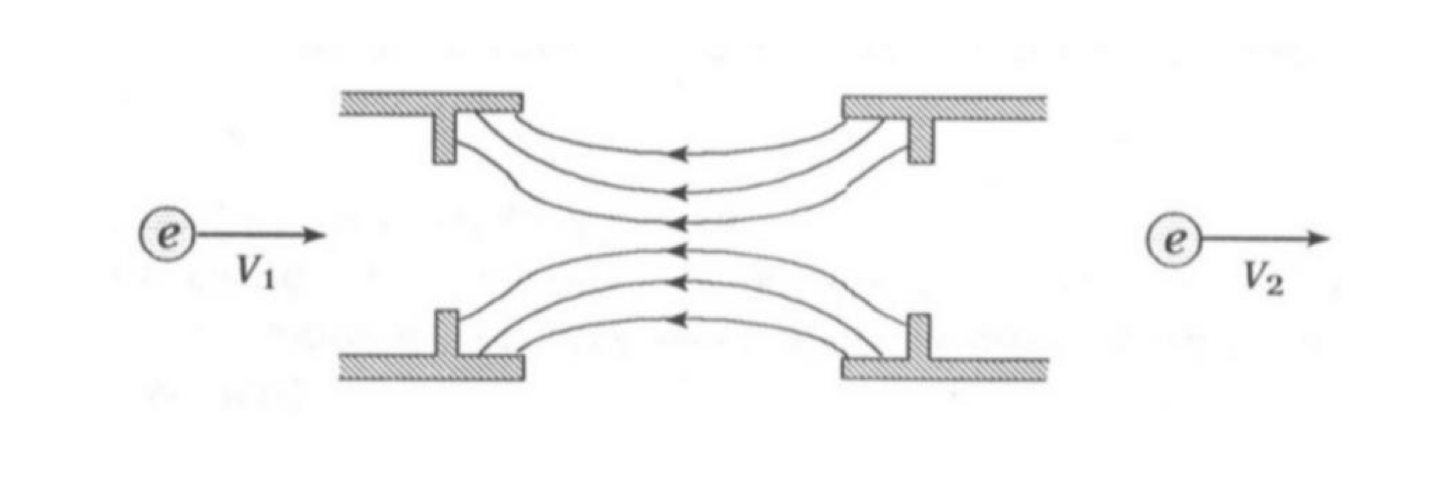
\includegraphics[width=0.5\linewidth]{electrostatic lens.png}
  \caption{Electrostatic lens}
  \label{fig:lens}
\end{figure}

\begin{figure}[H]
  \centering
  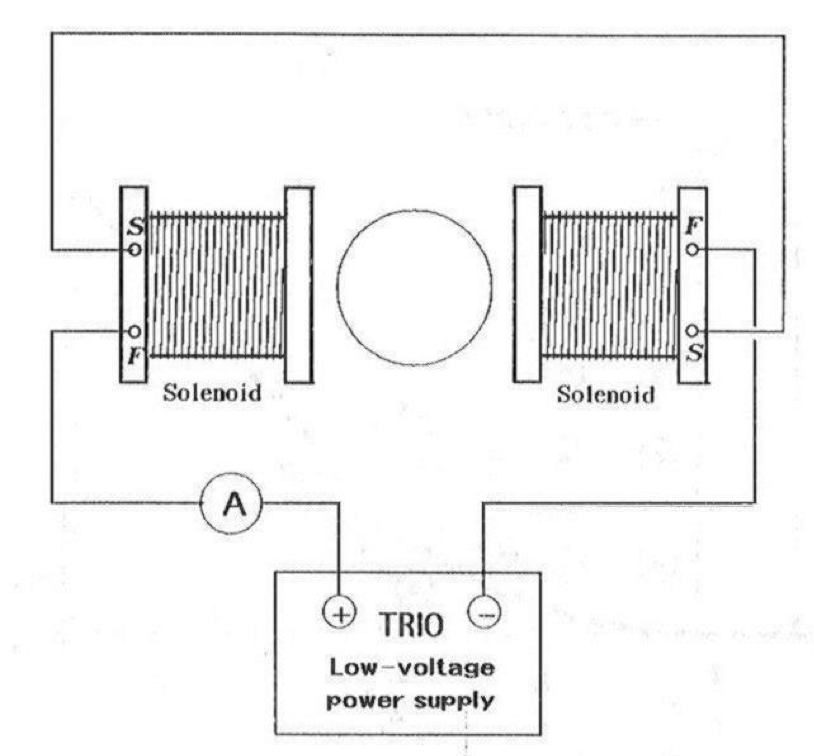
\includegraphics[width=0.5\linewidth]{magnetic system.png}
  \caption{Magnetic system}
  \label{fig:magnetic_system}
\end{figure}

\begin{figure}[H]
  \centering
  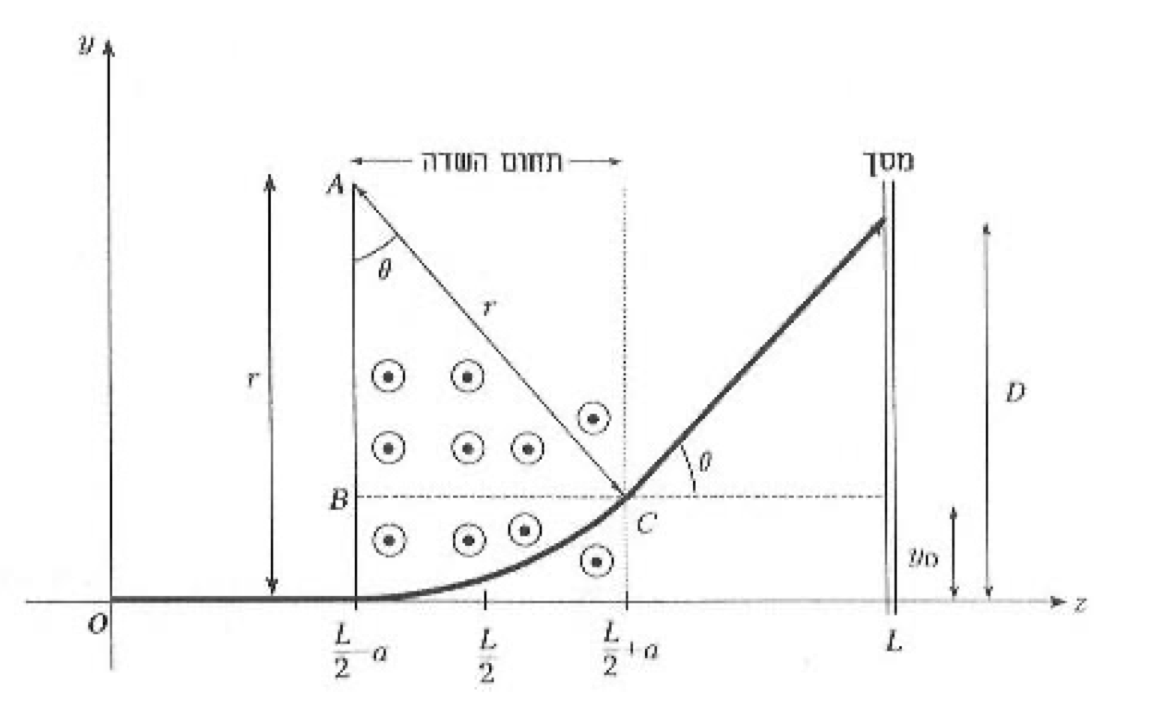
\includegraphics[width=0.5\linewidth]{electron path in a magnetic field.png}
  \caption{Electron path in a magnetic field}
  \label{fig:electron_path}
\end{figure}

% Subfigure sets, in order:
\begin{figure}[H]
  \centering
  \begin{subfigure}[b]{0.45\textwidth}
    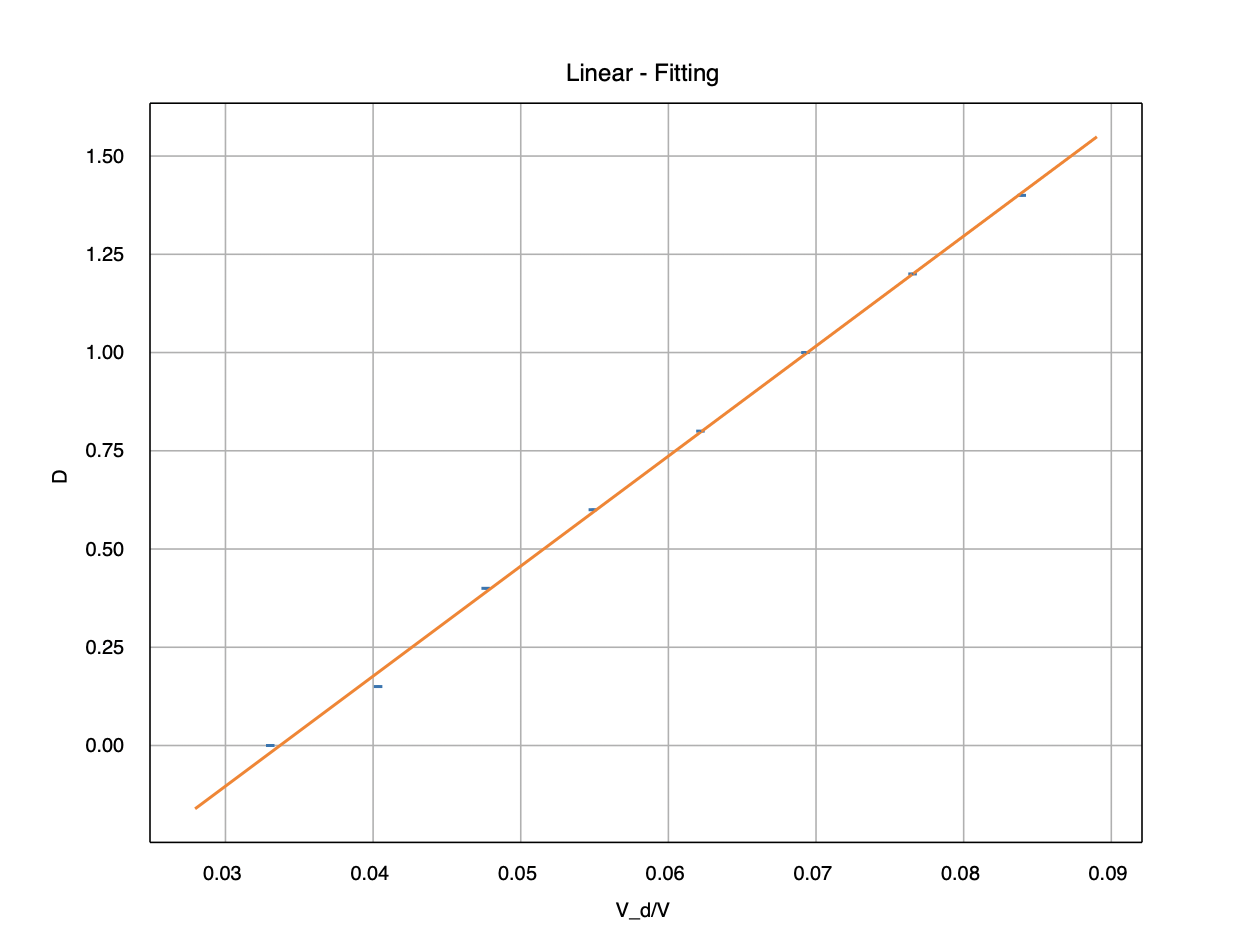
\includegraphics[width=\textwidth]{Electric measurments/first set fit.png}
    \caption{Linear fit}
    \label{fig:first_set_fit}
  \end{subfigure}\hfill
  \begin{subfigure}[b]{0.45\textwidth}
    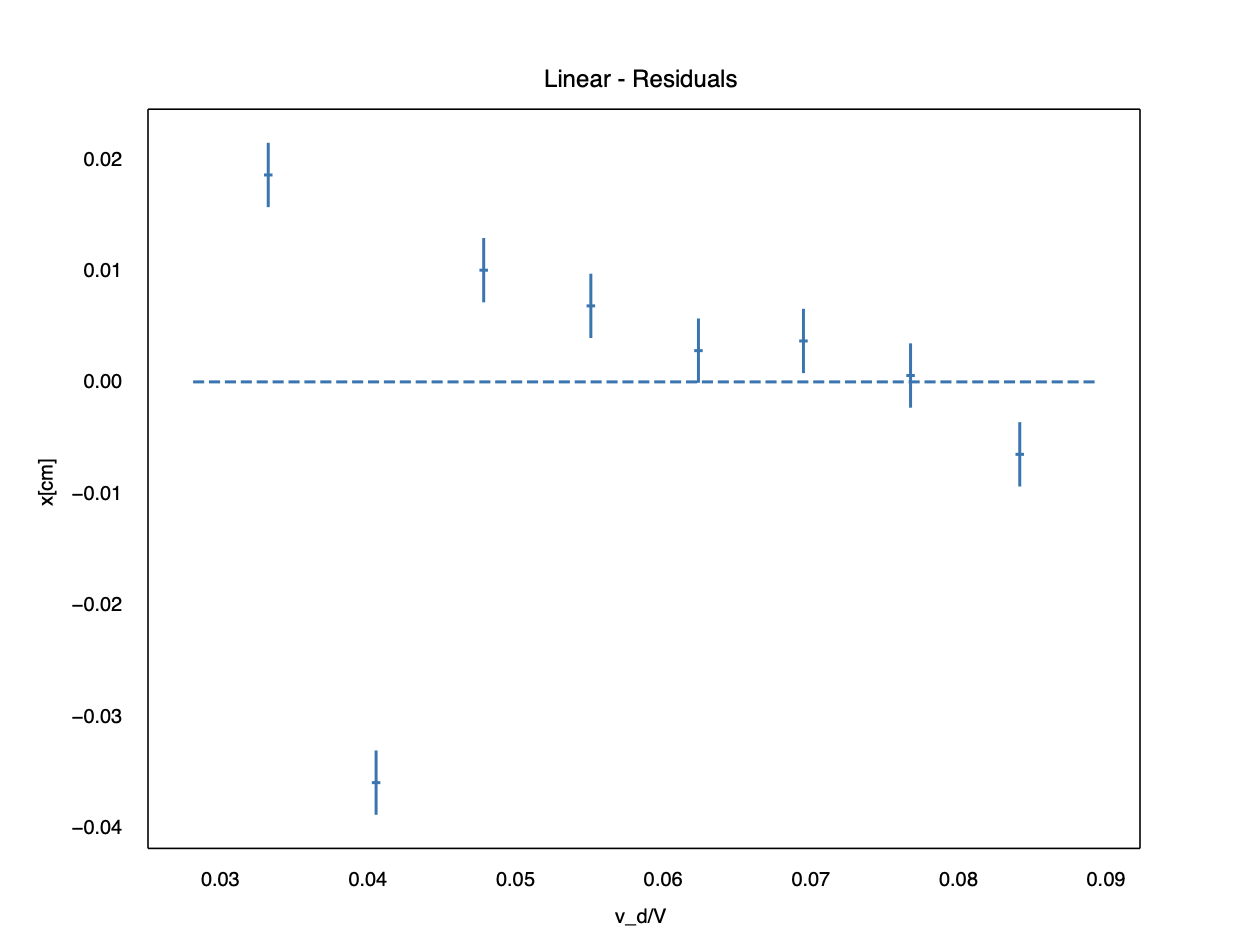
\includegraphics[width=\textwidth]{Electric measurments/first set residual.png}
    \caption{Residuals}
    \label{fig:first_set_residual}
  \end{subfigure}
  \caption{First set of measurements}
  \label{fig:first_set}
\end{figure}

\begin{figure}[H]
  \centering
  \begin{subfigure}[b]{0.45\textwidth}
    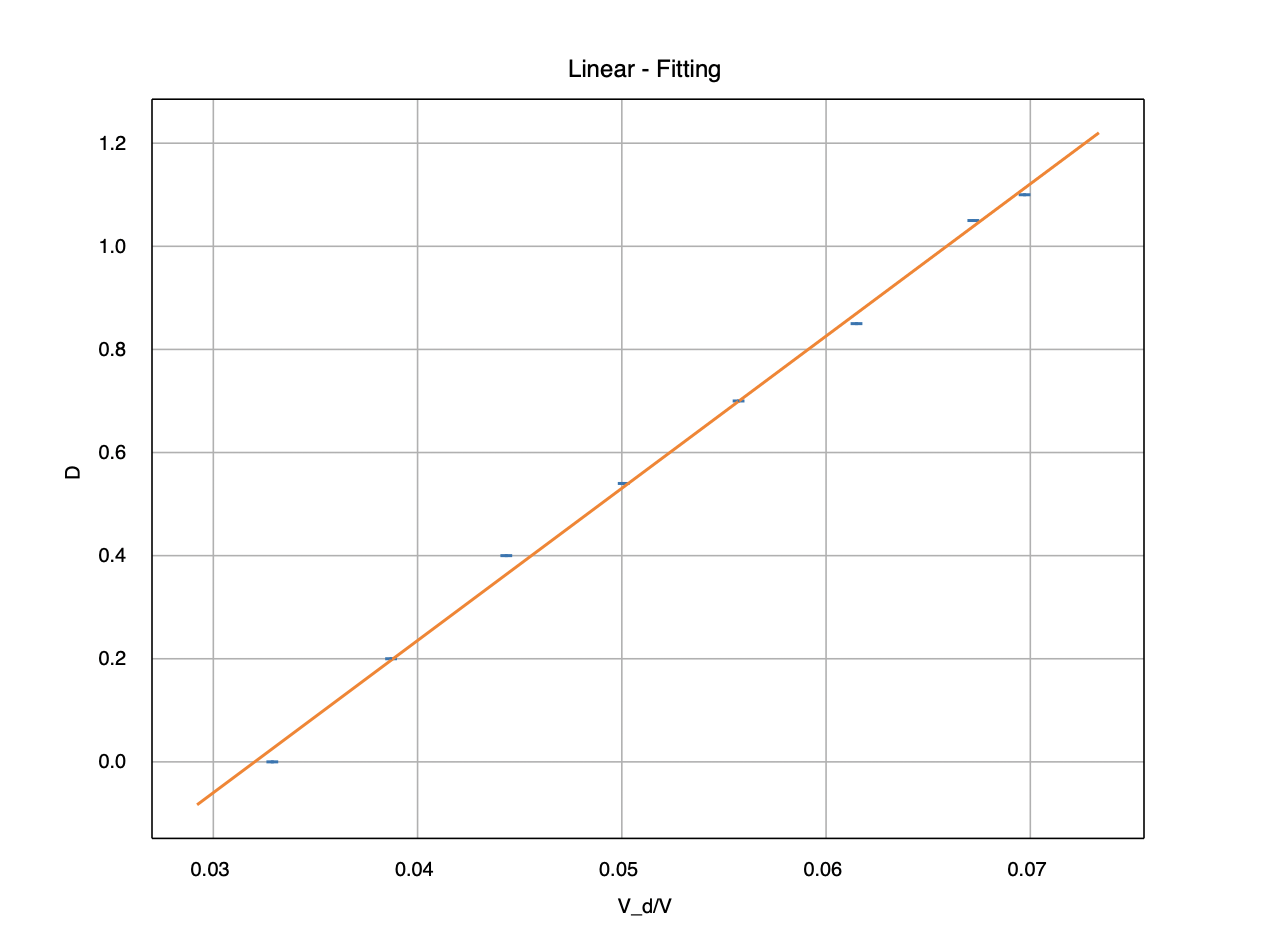
\includegraphics[width=\textwidth]{Electric measurments/second set fit.png}
    \caption{Linear fit}
    \label{fig:second_set_fit}
  \end{subfigure}\hfill
  \begin{subfigure}[b]{0.45\textwidth}
    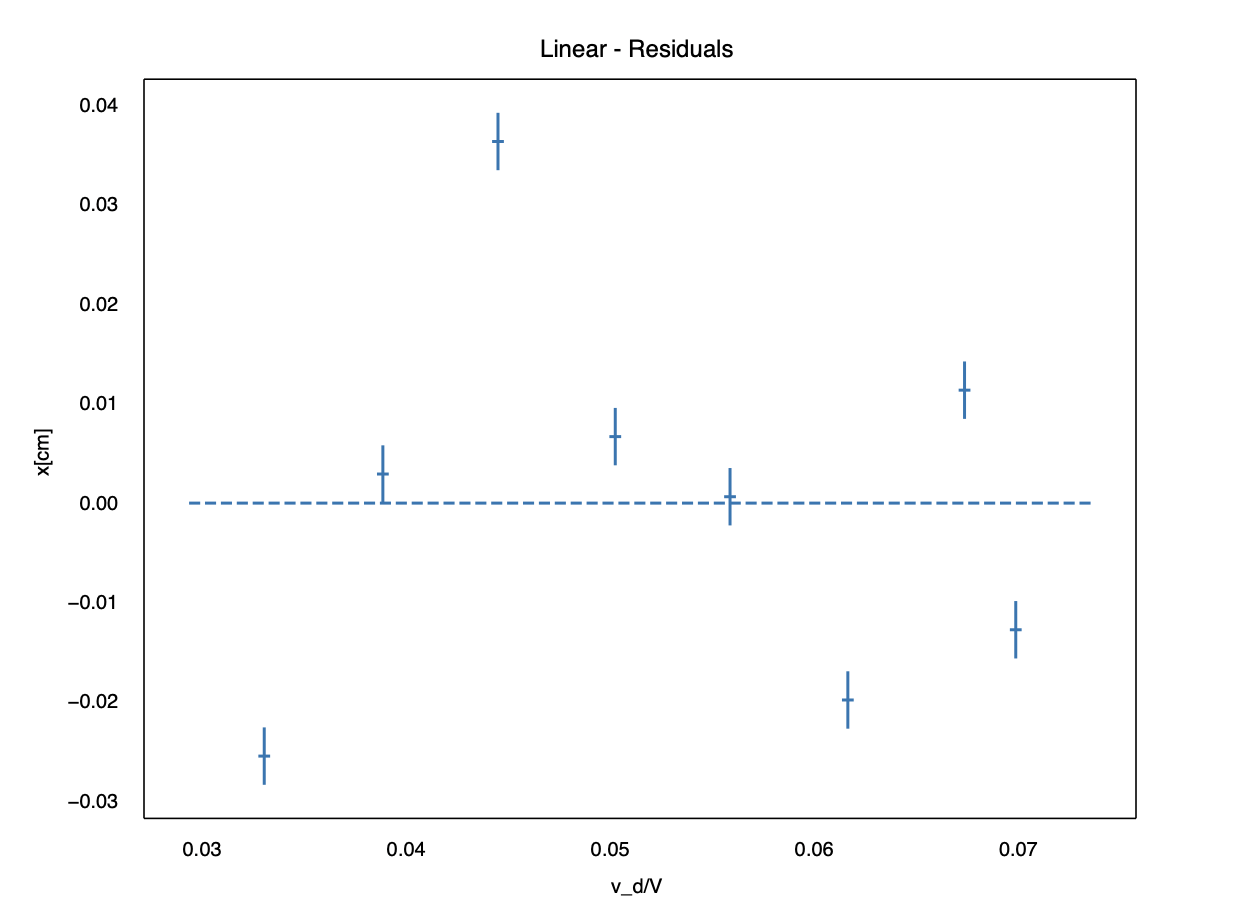
\includegraphics[width=\textwidth]{Electric measurments/second set residual.png}
    \caption{Residuals}
    \label{fig:second_set_residual}
  \end{subfigure}
  \caption{Second set of measurements}
  \label{fig:second_set}
\end{figure}

\begin{figure}[H]
  \centering
  \begin{subfigure}[b]{0.45\textwidth}
    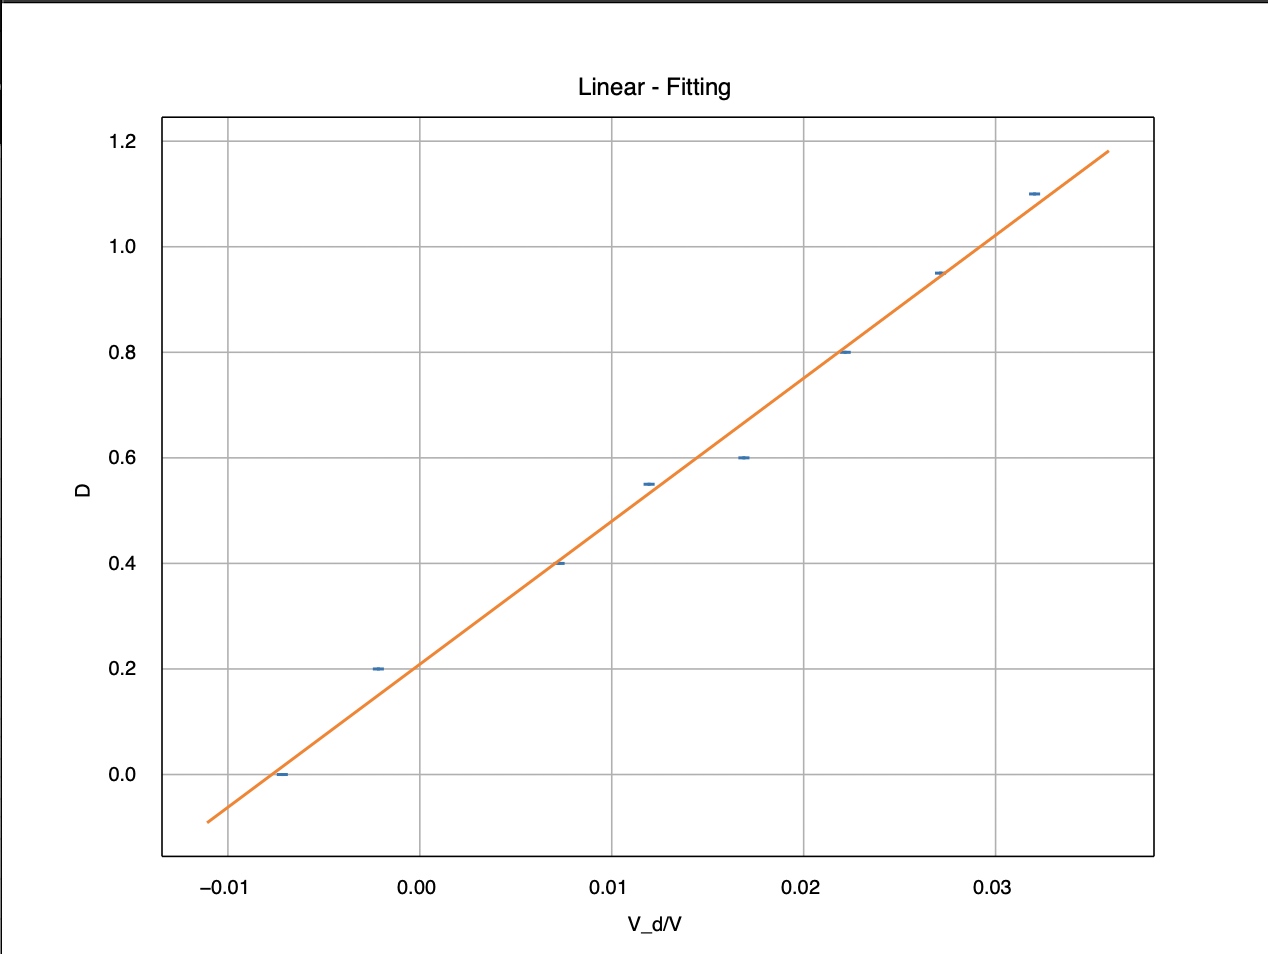
\includegraphics[width=\textwidth]{Electric measurments/Third set fit.png}
    \caption{Linear fit}
    \label{fig:third_set_fit}
  \end{subfigure}\hfill
  \begin{subfigure}[b]{0.45\textwidth}
    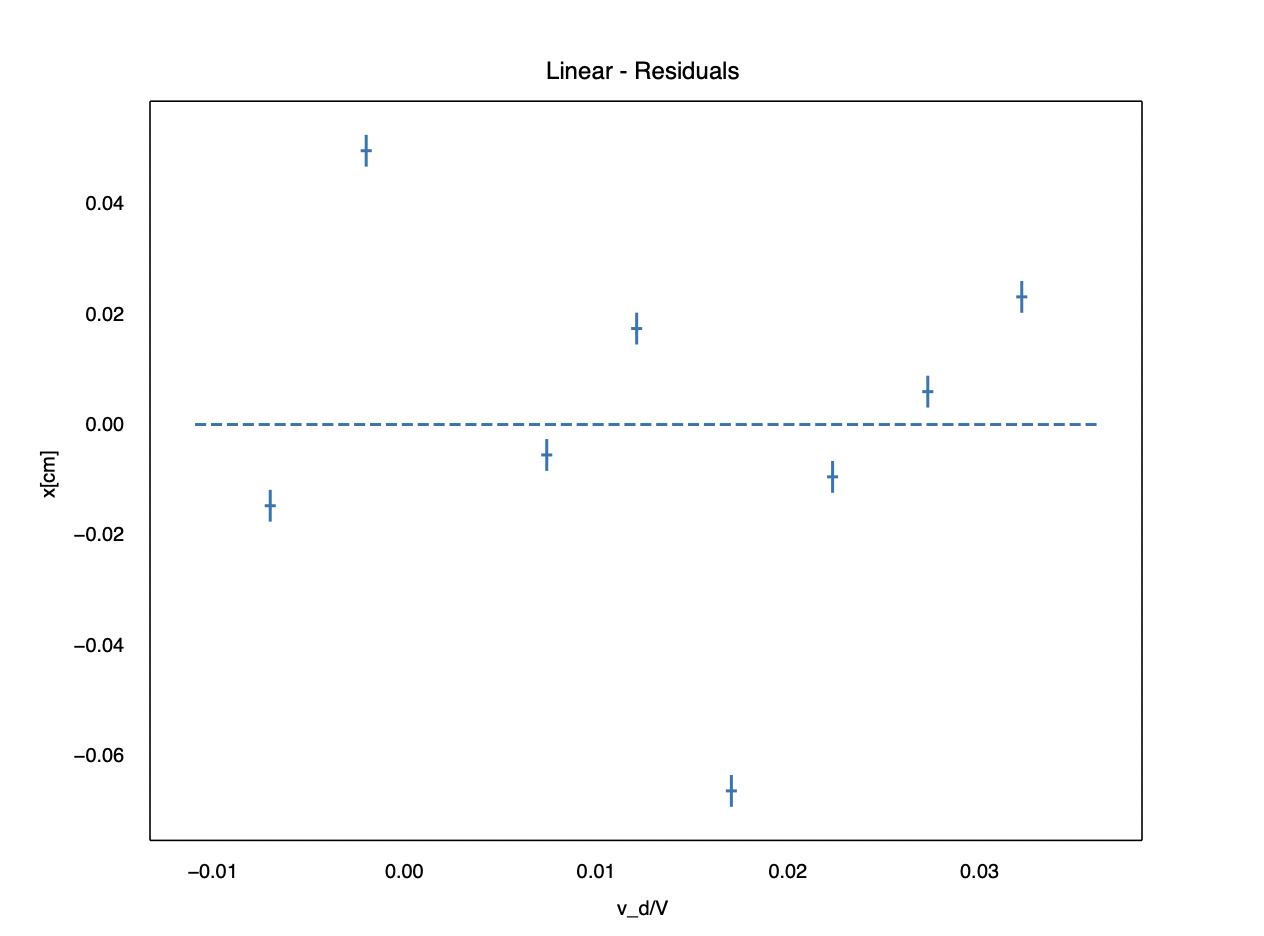
\includegraphics[width=\textwidth]{Electric measurments/Third set residual.png}
    \caption{Residuals}
    \label{fig:third_set_residual}
  \end{subfigure}
  \caption{Third set of measurements}
  \label{fig:third_set}
\end{figure}

% Force all figures out before starting tables
\clearpage

%====================================
\section{Tables Appendix}
\label{sec:tables_app}
\FloatBarrier

\begin{table}[H]
  \centering
  \begin{tabular}{|c|c|c|c|}
    \hline
    $\chi^2_{\mathrm{red}}$ & $p$-probability      & $a_0$             & $a_1$             \\ \hline
    4.184                   & $3.27\times10^{-4}$  & $-0.943\pm0.0227$ & $27.996\pm0.373$  \\ \hline
  \end{tabular}
  \caption{Results from the first set of measurements}
  \label{tab:first_set}
\end{table}

\begin{table}[H]
  \centering
  \begin{tabular}{|c|c|c|c|}
    \hline
    $\chi^2_{\mathrm{red}}$ & $p$-probability      & $a_0$             & $a_1$             \\ \hline
    5.574                   & $8.613\times10^{-6}$ & $-0.945\pm0.0324$ & $29.521\pm0.601$  \\ \hline
  \end{tabular}
  \caption{Results from the second set of measurements}
  \label{tab:second_set}
\end{table}

\begin{table}[H]
  \centering
  \begin{tabular}{|c|c|c|c|}
    \hline
    $\chi^2_{\mathrm{red}}$ & $p$-probability            & $a_0$              & $a_1$             \\ \hline
    19.40                   & $9.218\times10^{-23}$      & $0.208\pm0.0188$   & $27.097\pm1.011$  \\ \hline
  \end{tabular}
  \caption{Results from the third set of measurements}
  \label{tab:third_set}
\end{table}

\FloatBarrier
\end{document}
